% A mindmap showing TeX online projects supported
% by DANTE e.V. which sponsors their server costs.
% Author: Stefan Kottwitz
\documentclass[border=10pt]{standalone}
\usepackage[utf8]{inputenc}
\usepackage{dtklogos}
\usepackage{tikz}
\usetikzlibrary{mindmap,shadows}
\usepackage[hidelinks,pdfencoding=auto]{hyperref}
% Information boxes
\newcommand*{\info}[4][16.3]{%
  \node [ annotation, #3, scale=0.65, text width = #1em,
          inner sep = 2mm ] at (#2) {%
  \list{$\bullet$}{\topsep=0pt\itemsep=0pt\parsep=0pt
    \parskip=0pt\labelwidth=8pt\leftmargin=8pt
    \itemindent=0pt\labelsep=2pt}%
    #4
  \endlist
  };
}
\begin{document}
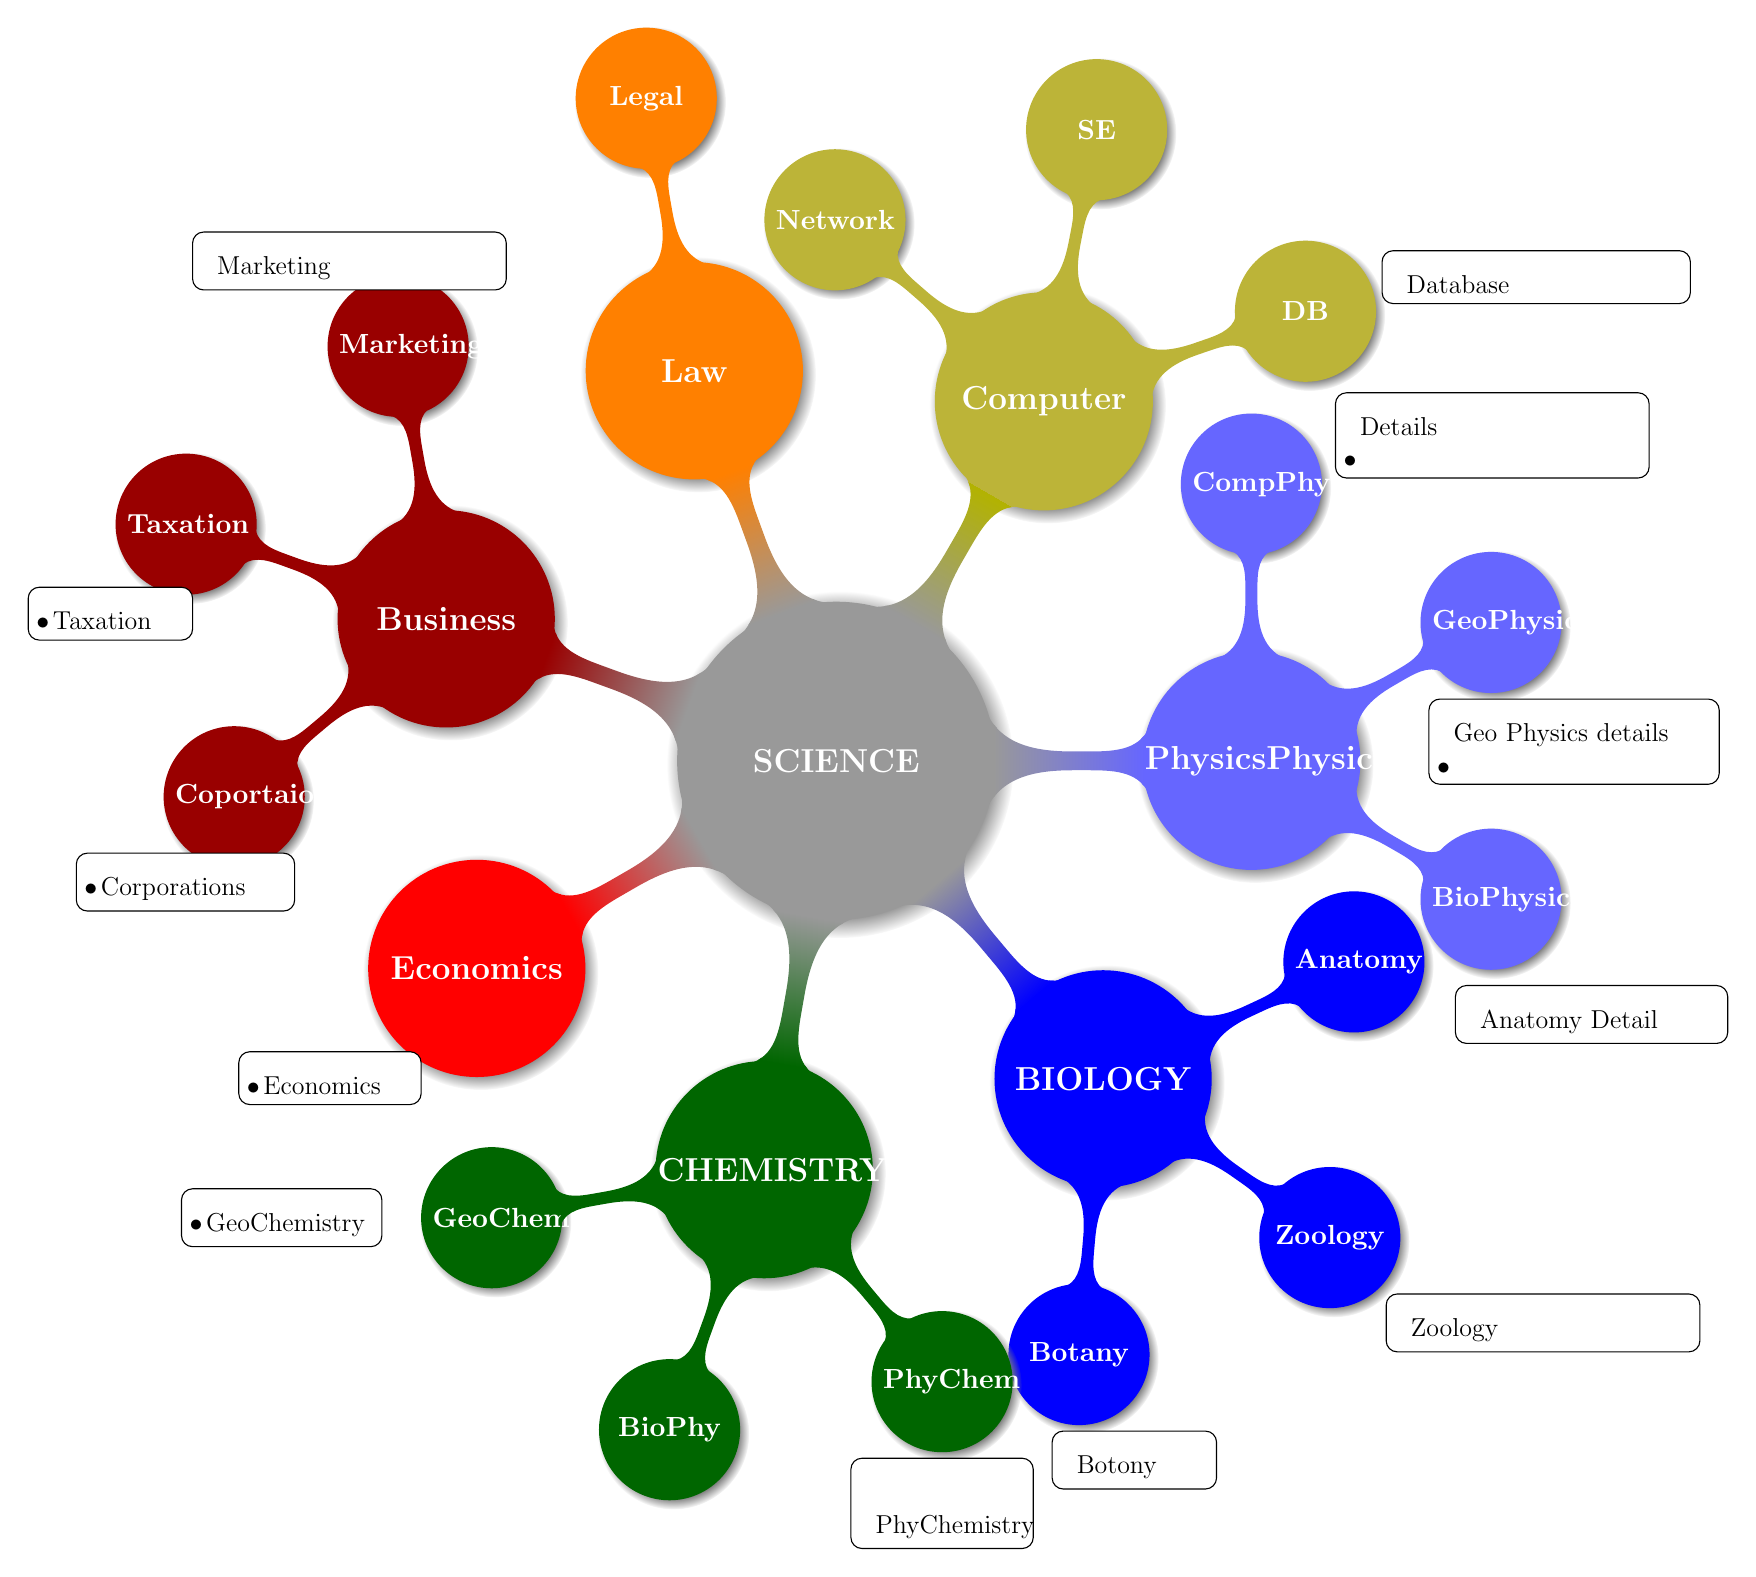
\begin{tikzpicture}[ every annotation/.style = {draw,
                     fill = white, font = \Large}]
  \path[mindmap,concept color=black!40,text=white,
    every node/.style={concept,circular drop shadow},
    root/.style    = {concept color=black!40,
      font=\large\bfseries,text width=10em},
    level 1 concept/.append style={font=\large\bfseries,
      sibling angle=50,text width=7.7em,
    level distance=15em,inner sep=0pt},
    level 2 concept/.append style={font=\bfseries,level distance=10em},
  ]
  node[root] {SCIENCE} [clockwise from=0]
    child[concept color=blue!60] {
      node {\href{Physics}{Physics}} [clockwise from=90]
        child { node (goForum) {{CompPhysics}} }
        child { node (goWiki) {{GeoPhysics}} }
        child { node (BioPhy) {{BioPhysics}} }
    }
    child[concept color=blue] {
      node[concept] {{BIOLOGY}}
        [clockwise from=25]
      child { node[concept] (TeXnique)
        {{Anatomy}} }
      child { node[concept] (TeXweltQA)
        {{Zoology}} }
      child { node[concept] (TeXweltBlog)
        {{Botany} }}
    }
    child[concept color=green!40!black] {
      node[concept] {{CHEMISTRY}}
        [clockwise from=310]
      child { node[concept] (TikZGalerie) 
        {{PhyChem}} }
      child { node[concept] (TeXampleBlog)
        {{BioPhy}} }
      child { node[concept] (Planet)
        {{GeoChem}} }
    }
    child[concept color=red] {
      node[concept] (PGFPlots) {{Economics}}
      [clockwise from=270]
    }
    child[concept color=red!60!black] {
      node[concept] {{Business}}
        [counterclockwise from=100]
      child { node[concept] (LaTeXForum)
        {{Marketing}}}
      child { node[concept] (LaTeXArtikel)
        {{Taxation}} }
      child { node[concept] (LaTeXNews)
        {{Coportaions}} }
    }
    child[concept color=orange] {
      node[concept] (TeXdoc)
        {{Law}}
        [clockwise from=100]
        child { node[concept] {{Legal}}
        }}
    child[concept color=yellow!70!black] {
      node[concept] (Blogs) {Computer} [clockwise from=139]
      child { node[concept] {{Network}}}
      child { node[concept] {SE}}
      child { node[concept] (Cookbook){DB}}
%      child { node[concept] (Cookbook){CA}}
    };
    \info{goForum.north east}{above,anchor=west,xshift=1em}{%
      \item[] Details
      \item 
    }
    \info{LaTeXForum.north west}{above,anchor=south}{%
      \item[] Marketing
    }
    \info[8]{LaTeXArtikel.west}{below,anchor=north east,xshift=3em,yshift=-2em}{%
      \item Taxation
    }
    \info[11]{LaTeXNews.south west}{below,anchor=north}{%
      \item Corporations
    }
    \info[9]{TikZGalerie.south}{below,anchor=north}{%
      \item[] PhyChemistry
    }
    \info[15]{goWiki.south}{below,anchor=north,xshift=3em}{%
      \item [] Geo Physics details
      \item
    }
    \info{TeXweltQA.south east}{above,anchor=north west}{%
      \item[] Zoology
    }
    \info[8]{TeXweltBlog.south}{below,anchor=north,xshift=2em}{%
      \item[] Botony
    }
    \info[9]{PGFPlots.south west}{anchor=north east,xshift=1em}{%
      \item Economics
    }
    \info[10]{Planet.west}{anchor=east,xshift=-1.2em}{%
      \item GeoChemistry
    }
    \info[14]{TeXnique.east}{anchor=west,xshift = 0.9em,yshift=-1.9em}{%
      \item[] Anatomy Detail
    }
    \info[16]{Cookbook.east}{anchor=south west}{%
      \item[] Database
    }
\end{tikzpicture}
\end{document}